\documentclass[12pt,a4paper]{journal}
\usepackage[margin=1in]{geometry}

\usepackage[utf8]{inputenc}
\usepackage[T1]{fontenc}
\usepackage{indentfirst}
\usepackage{amsmath}
\usepackage{amsfonts}
\usepackage{amssymb}
\usepackage{caption}
\usepackage{subcaption}
\usepackage{graphicx}
\usepackage{siunitx}
\sisetup{range-phrase=--, range-units=single}

\graphicspath{{img/}}
\usepackage[numbers, square]{natbib}


\begin{document}

\subsection{Physiology of the retina}

Images to include:
\begin{itemize}
\item diagram of the organization of the eye (overall structure)
\item diagram/picture of the organization of the retinal layers
\item images of healthy retinal scans (structural/angiogram)
\end{itemize}

\subsubsection{In health}

\begin{itemize}
\item organization of the eye: iris/lens..., vitreous, retina, choroid, sclera
\item organization of the retina: optic nerve head, macula, fovea, the difference layers of cells
\item how each layer is attached to each other
\item how incoming light is processed: travels through the retina, captured by photoreceptors, transformed in biochemical signal, transform in elecrtical signal, sent through the optic nerve to the brain
\item the vasculature in the retina and the choroid (add where it comes from, i.e., ophthalmic artery?)
\item ajouter des images de healthy/diseased retinae OCTA/FA and OCT
\item role du RPE
\end{itemize}

\large\textbf{organization of the eye: iris/lens..., vitreous, retina, choroid, sclera}

The retina is a layer of tissue, aproximately \SI{0.5}{\mm} thick, that lines the back of the eye.
The retinal inner surface is attached to the vitreous body, the clear gel that separates the lens and the retina, while its outer surface is attached to Bruch's membrane, see Figure~\ref{fig:architecture-eye}.
When looking at a cross section of the retina as shown in Figure~\ref{fig:architecture-eye}, eight layers can be identified, the innermost (closest to the vitreous) being the nerve fiber layer and the outermost the retinal pigmented epithelium (RPE).
In the centre of the retina is a oval-shaped pigmented area called the macula.

The macula is about \SI{5}{\mm} wide and is responsible for the highly detailed, central vision thanks to its high concentration of photoreceptor cells, namely rods and cones.
In particular, cones are highly concentrated in the centre of the macula, in a pit approximately \SI{1.5}{\mm} wide named the fovea.
The fovea is a critical area of the retina, with a number of conditions appearing at or around it.
\\
Another important structure of the retina in disease is the optic disc.
The optic disc appears as a round spot on \textit{en-face} views of the retina and is around \SI{1.8}{\mm} wide.
Through the optic disc passes the optic nerve, the fibers of which extend to form the nerve fiber layer, which transmits visual information to the brain.

%% 
% Light hitting the retina travels through the retinal thickness to reach the photoreceptor layer, located just above the RPE.
Visual information originates from light hitting the retina.
The light crosses the retinal thickness to reach the body of the photoreceptors, in the layer just before the RPE.
%%
Activation of photoreceptors by photon starts a cascade of biochemical reactions the transform light into a biochemical signal~\cite{Hurley2009}.
This biochemical signal is picked up by cells in the inner layers of the retina, which transform it into an electrical signal~\cite{Arslan2018}.
The electrical signal is then transmitted to the nerve fiber layer, which relays it to the brain via the optic nerve, enabling vision.

Owing to its pigmentation, the RPE acts as a buffer for remaining lights, protecting the retina from light damage and preventing backreflection of light that may interfer with the visual outcome.
The RPE is formed of a single layer of epithelial cells, which primary function is to support photoreceptors.
To fulfill this purpose, the RPE acts as the blood-retinal barrier, hence regulating the transport of ions, fluid, proteins and other molecules~\cite{Boulton2001}.
The photoreceptors are attached to the RPE cells plasma membrane.
Through this close interaction, the RPE collects by-products of the photoreceptors, an essential action to maintain visual function.
Those by-products are released into the systemic circulation via the choroid, one of the two circulations of the retina~\cite{Boulton2001}.

Visual functions require high metabolic activity from the retinal cells, which makes the retinal tissue very demanding in oxygen.
In fact, the rates of oxygen consumption per unit volume of tissue are comparable for the brain and the retina~\cite{Medrano1995}.
To sustain the demand in oxygen, the retina is equiped with a dense network of capillaries, that branches out of the central retinal artery (CRA) and finishes at the central retinal vein (CRV).
The CRA is a branch of the ophthalmic artery and the CRV drains into the superior ophthalmic vein.
Both the CRA and CRV enter and exit the retina along the optic nerve.
The CRA's branches spread across four plexi within the inner half of the retinal depth, namely, the superficial (SCP), intermediate (ICP), deep (DCP) and the radial peripapillary capillary plexus (RPCP).
%%
%The aggregation of adjacent plexi leads to the use of the terms superficial vascular complex (SVC) and deep vascular complex (DVC).
%%
The terms superficial vascular complex (SVC) and deep vascular complex (DVC) are sometimes used to designate the RPCP-SCP complex and the ICP-DCP complex, respectively.

The inner retinal circulation provides oxygen for the inner \SIrange{60}{80}{\percent} of the tissue.
The perfusion of the remaining outer \SIrange{20}{40}{\percent} is covered by the choroid.
The choroid is a vascular tissue of the eye that lies beinhd the RPE, from which it is separated by Bruch's membrane, a thin (\SIrange{2}{4}{\micro\meter}), permeable barrier that provides structural support to the RPE and regulates gas and mass exchanges with the choroid~\cite{Curcio2013}.

%%
%Bruch's membrane is a thin (\SIrange{2}{4}{\micro\meter}), permeable barrier that controls exchanges of gas, nutrients and byproducts of metabolic activity between the RPE and the choroid~\cite{Curcio2013}. 
%
The choroid is structured in three vascular layers.
From the outermost to the innermost: Haller's layer, Sattler's layer and the choriocapillaris (CC).
The diameter of the vessels in each layer decreases as it approaches the retina, with the CC only composed of capillaries.
The vascular input to the choroid is provided by the short posterior ciliary arteries (between 6 and 12), which are branches of the ophthalmic artery~\cite{Kiel2010}.
The large vessels of the two outer layers of the choroid run parallel to the retinal axis.
Some arterioles from Sattler's layer branch at an almost \SI{90}{\degree} angle to perfuse the CC~\cite{Nickla2010}.
Each of these arterioles form an hexagonal-shaped domain, fed by a single arteriole and drained by a varying number of venules back into Sattler's layer~\cite{Zouache2016}.
The capillaries of the CC have wide lumen (the cavity delimited by the vessel's walls), between \SIrange{7}{40}{\micro\meter} in the CC against \SIrange{5}{10}{\micro\meter} in the retina, and are arranged into a single plane, with many connection between adjacent capillaries, also known as anastomosis~\cite{Bill1983, ChanLing2011,Fryczkowski1994}.
Furthermore, the capillary walls have opening (or fenestration), increasing their permeability~\cite{Nickla2010}.
The fenestrations on the capillary walls are more numerous on the side facing the retina and are at least wide enough to let molecules with a diffusional radius of \SI{3.7}{\micro\meter} pass into the blood~\cite{Nickla2010, Bill1983}.
This particular architecture combined with a high blood flow allows the CC to provide enough oxygen through difusion across Bruch's membrane and the outer retina and clear wastes from the retina towards the systemic circulation.

The blood supply from the choroid to the outer retina is indirect.
Therefore, the choroid has high blood flow and a high oxygen content~\cite{Bill1983}.
The high concentration of oxygen in the choroidal circulation creates a strong gradient for its diffusion between the choriocapillaris and the outer retina.
The high blood flow rates may help regulating the temperature of the macula, by keeping it at the same temperature as the rest of the body~\cite{Bill1983, Parver1991}.

While appropriate blood supply is necessary to maintain vision, blood vessels can interfere with light and hinder resulting images.
The distribution of photoreceptor in the retina is heterogeneous, with a higher concentration in the parafovea, for rods, and fovea, for cones~\cite{Zouache2022}.
For this reason, the centre of the fovea is an avascular zone around \SI{500}{\micro\meter} wide, often refered to as the foveolar avascular zone (FAZ).




\begin{figure}[h]
  \centering
  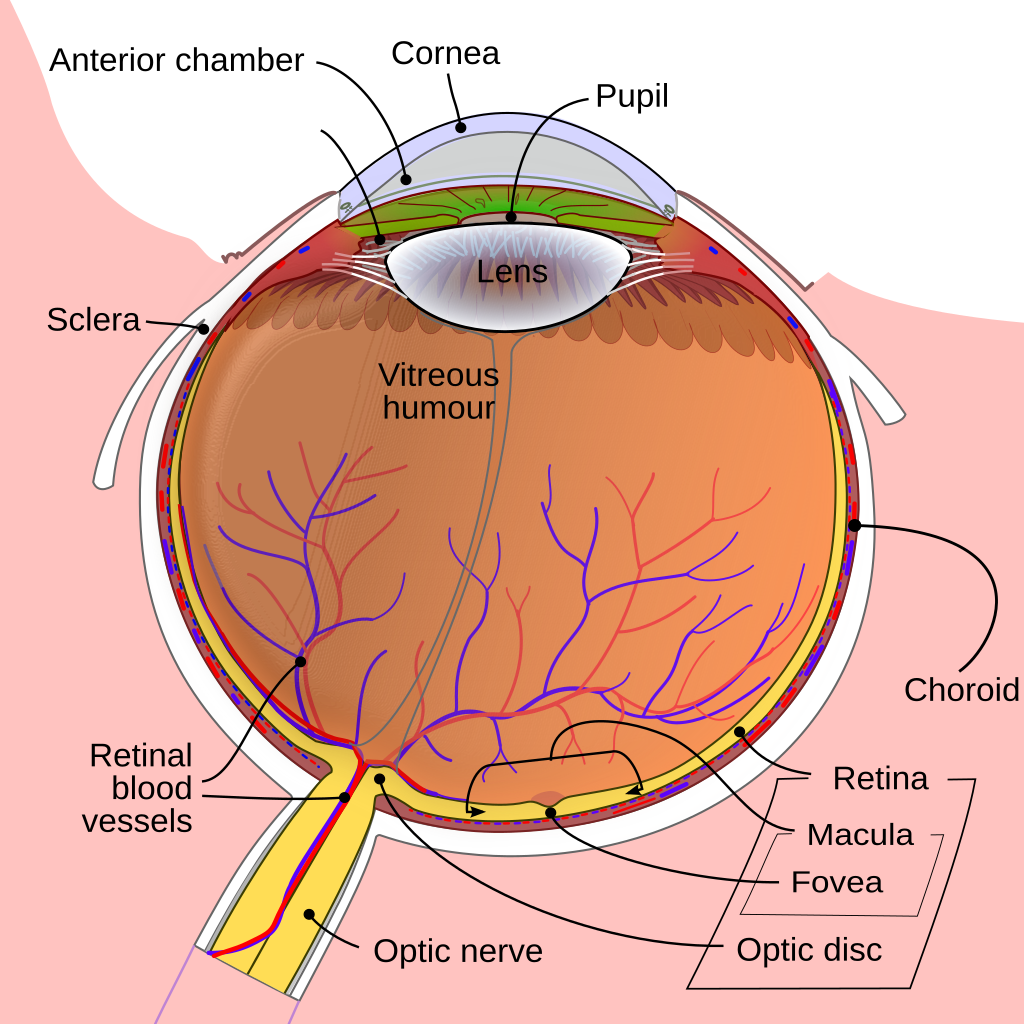
\includegraphics[width=0.45\textwidth, height=7cm]{ArchitectureEye} % From Wikipedia retina
  \hfill
  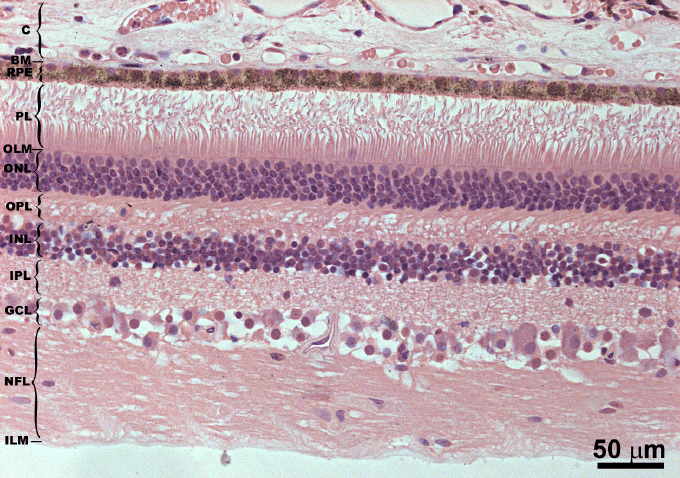
\includegraphics[width=0.45\textwidth, height=7cm]{RetinaHistology}
  \caption{General architecture of the eye and the retina. This is for illustration, taken from Wikipedia and 'Glia and blood retinal barrier: effects of ocular hypertension' and rights need to be checked/the pics need to be eddited.}
  \label{fig:architecture-eye}
\end{figure}
\subsubsection{In disease}

\begin{itemize}
\item degradation of the blood supply chain (rarefaction des vaisseaux sanguins dans la retine (e.g. en cas de diabete) et le choriocapillaris (e.g. AMD)
\item augmentation de la pression occulaire (IOP) in, e.g., glaucoma
\item epaississement de la membrane de Bruch avec l'age et peut-etre AMD?
\item formation de drusen in AMD et avec l'age et le risque de detachement de la retine ou du RPE
\item neovascularisation et leakages
\end{itemize}

% \begin{spacing}{0.0}
\bibliographystyle{abbrvnat} % {ksfh_nat}
{\normalsize \bibliography{section_2}}
% \end{spacing}

\end{document}
